% !TEX TS-program = pdflatexmk
\input{../pre.tex}
\usepackage{comment}
\usepackage{wrapfig}
\setlength{\columnsep}{0.7cm}
%\fontfamily{qcr}\selectfont 
%\usepackage[backend=bibtex]{biblatex}

\usepackage[
backend=biber,
style=alphabetic,giveninits,
citestyle=ieee-alphabetic,
natbib=true,
uniquelist=false,
maxnames=10,
sorting=ynt
]{biblatex}
%
\addbibresource{ref.bib}

\title{\textbf{Optimization for Machine Learning}\\ Lecture $1$ }
\usepackage{quiver}
\usepackage[nobottomtitles*]{titlesec}
\usepackage{titletoc}

\author{Nilava Metya}
\date{\vspace{-0.7in}January $23$, $2026$}
%\newcommand{\pb}{\section{Problem}~\par}
%\newcommand{\soln}{\subsection*{Solution}}
\usepackage{pdfpages}
\usepackage{fancyhdr}
	\pagestyle{fancyplain}
	\fancyhf{}
	\fancyhead[R]{\thepage}
\newcommand{\fa}{~\forall~}
\usepackage{algpseudocode}
\renewcommand{\algorithmicrequire}{\textbf{Input:}}
\renewcommand{\algorithmicensure}{\textbf{Output:}}
\algdef{SE}{Begin}{End}{\textbf{begin}}{\textbf{end}}
\begin{document}

\maketitle

\section{Introduction to optimization}
We write $$\min_{x\in \cX}f(x)$$ to denote an optimization problem where $x$ is a decision variable, $f(x)$ is the objective (cost) function to minimize, $\cX$ is the constriant set. If a point $x_{*}$ that minimizes $f$ then we call it an \textit{optimizer} and $f(x_{*})$ is the \textit{optimal value}.  

\section{Simple Regression (one predictor)}
Let $y$ be the output variable (house prices), $a$ be the input vector and $x$ is the decision variable. The loss function we consider is $L(x,y,a) = \frac12(y-(x_{1}+x_{2}a_{1}))^{2}$. 

Example: Say I have a dataset with $(y,a)$ as $\set{(0,0),(1,1)}$. The loss becomes $f(x) = L(x,0,0)+L(x,1,1) = \frac{x_{1}^{2} + \left[ 1-(x_{1}+x_{2}) \right]^{2}}2$. This $f(x)=0$ looks like a `cereal bowl'.
\begin{figure}[]
 \centering
  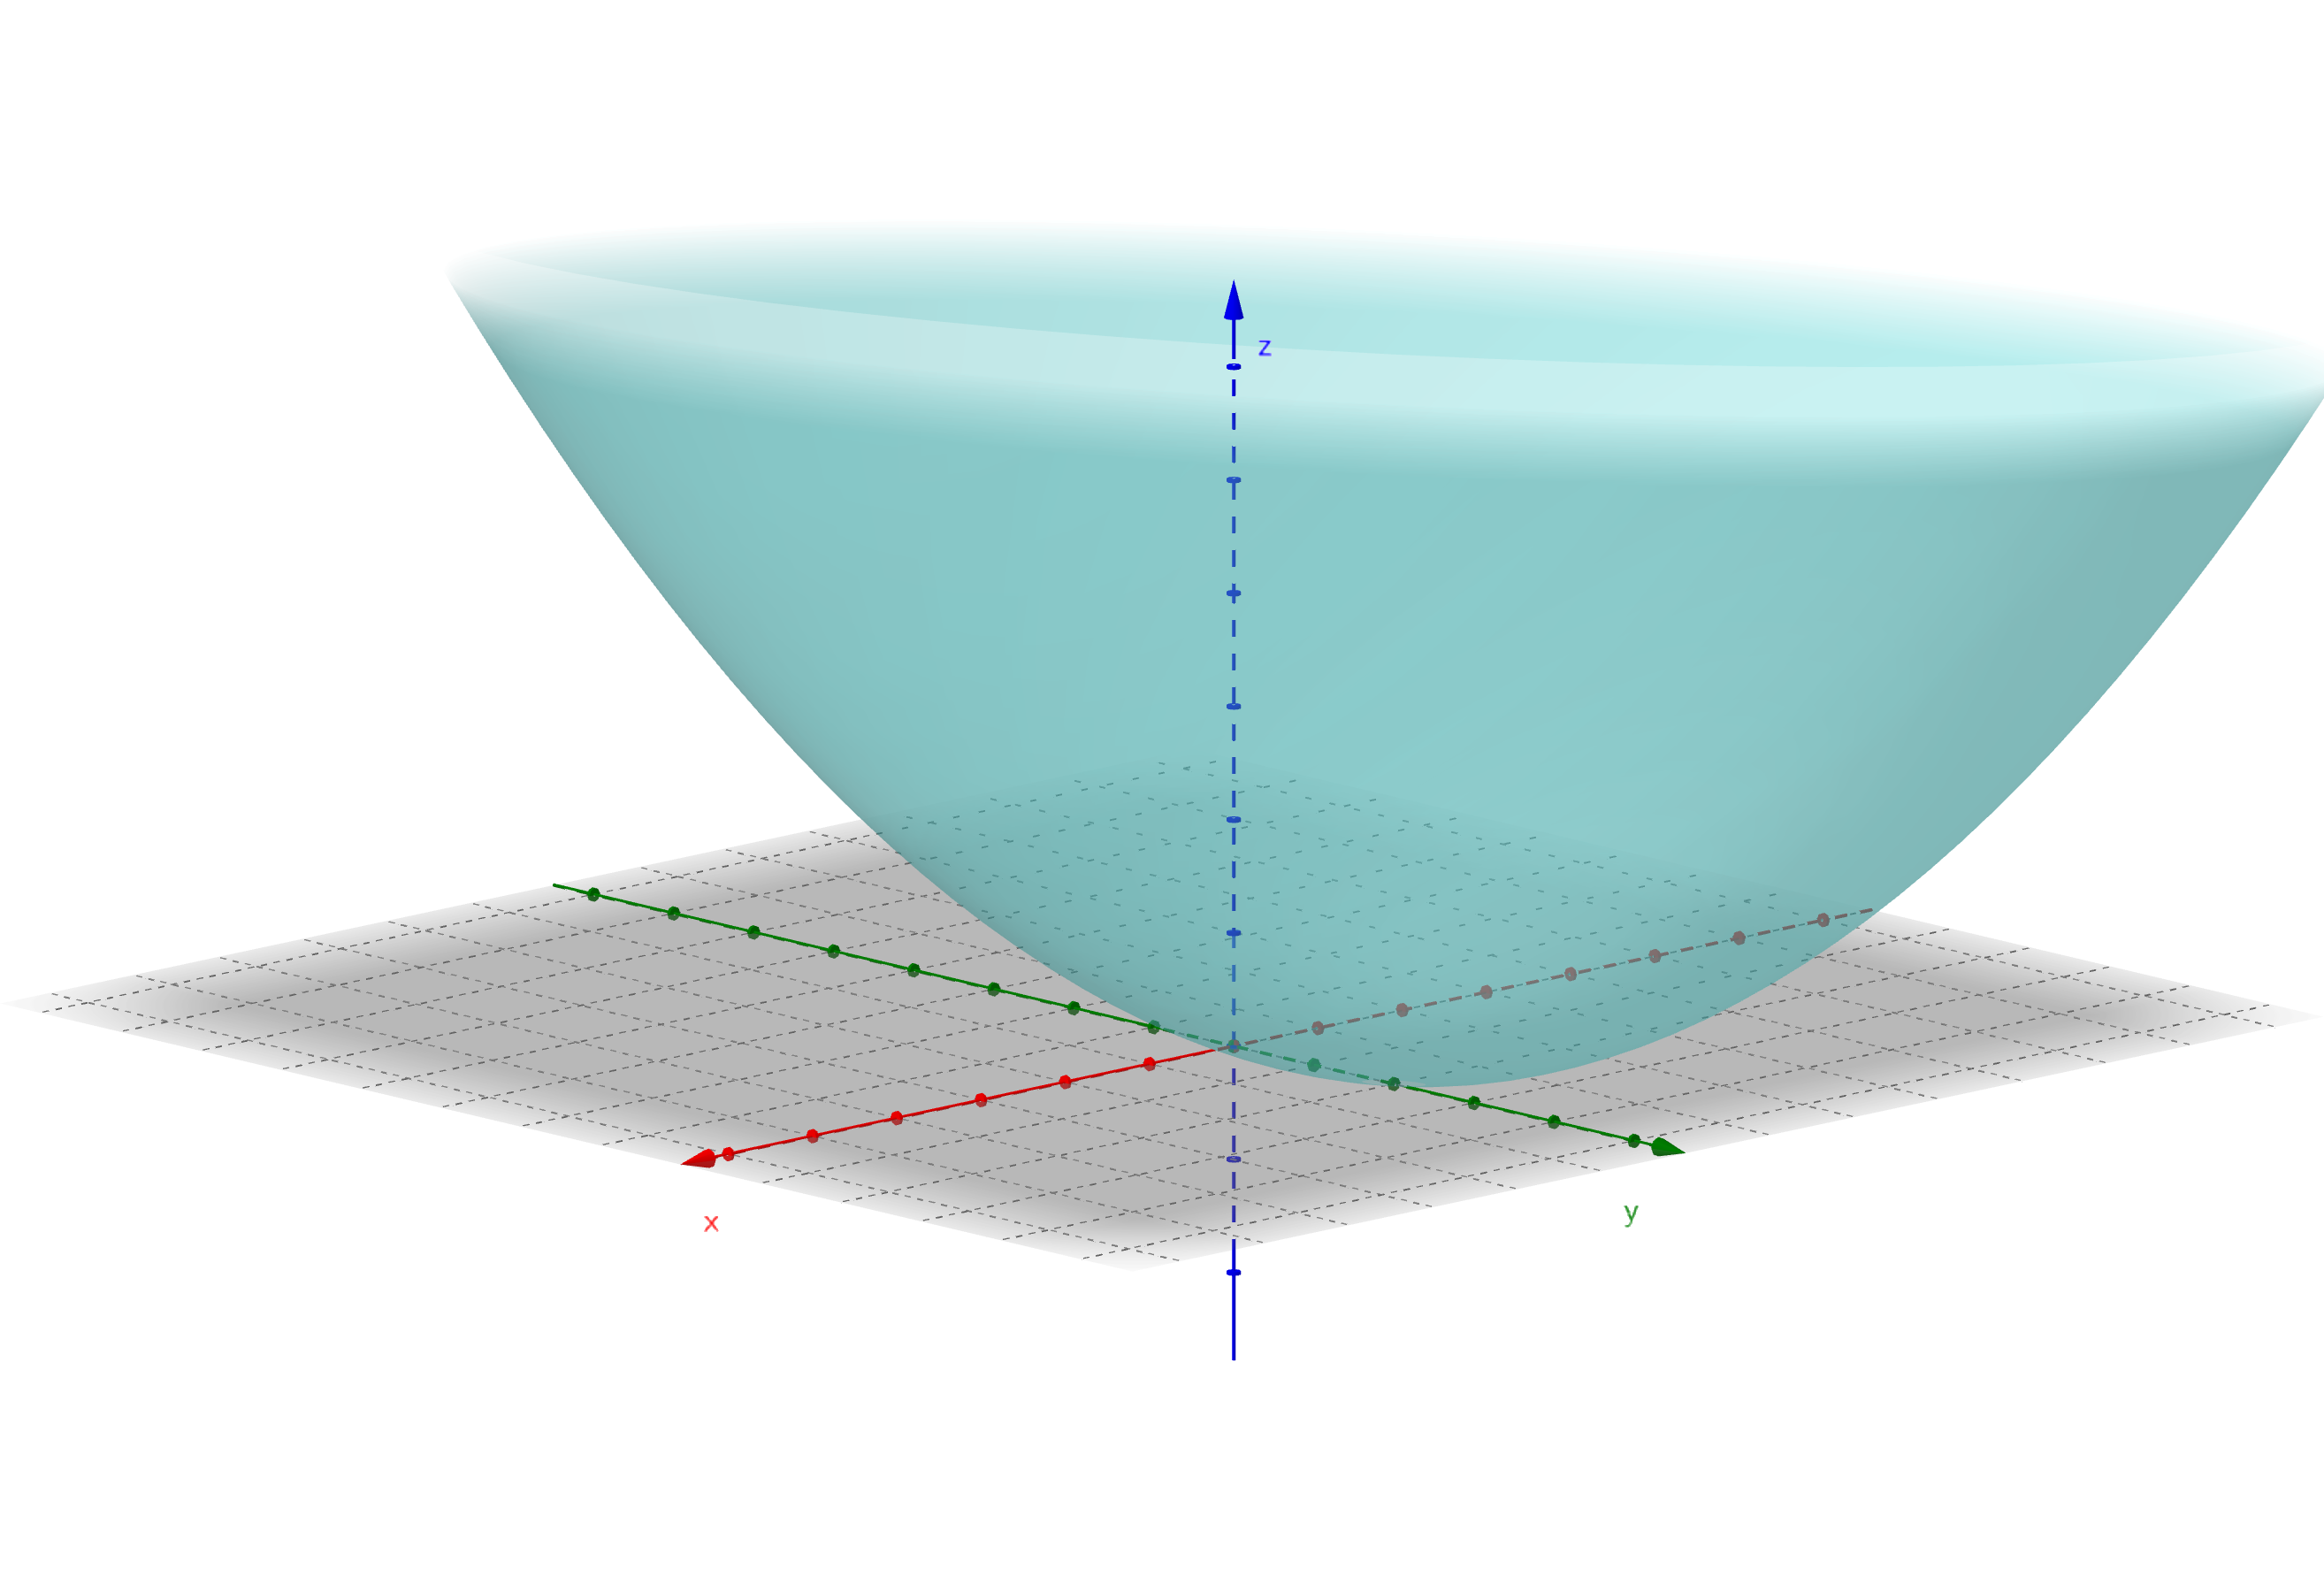
\includegraphics[width=0.5\textwidth]{bowl.png}
 \end{figure}
 


Level sets are sets of the form $L_{a}(f) = \set{x\st f(x)= a}$. 

\begin{figure}[]
 \centering
  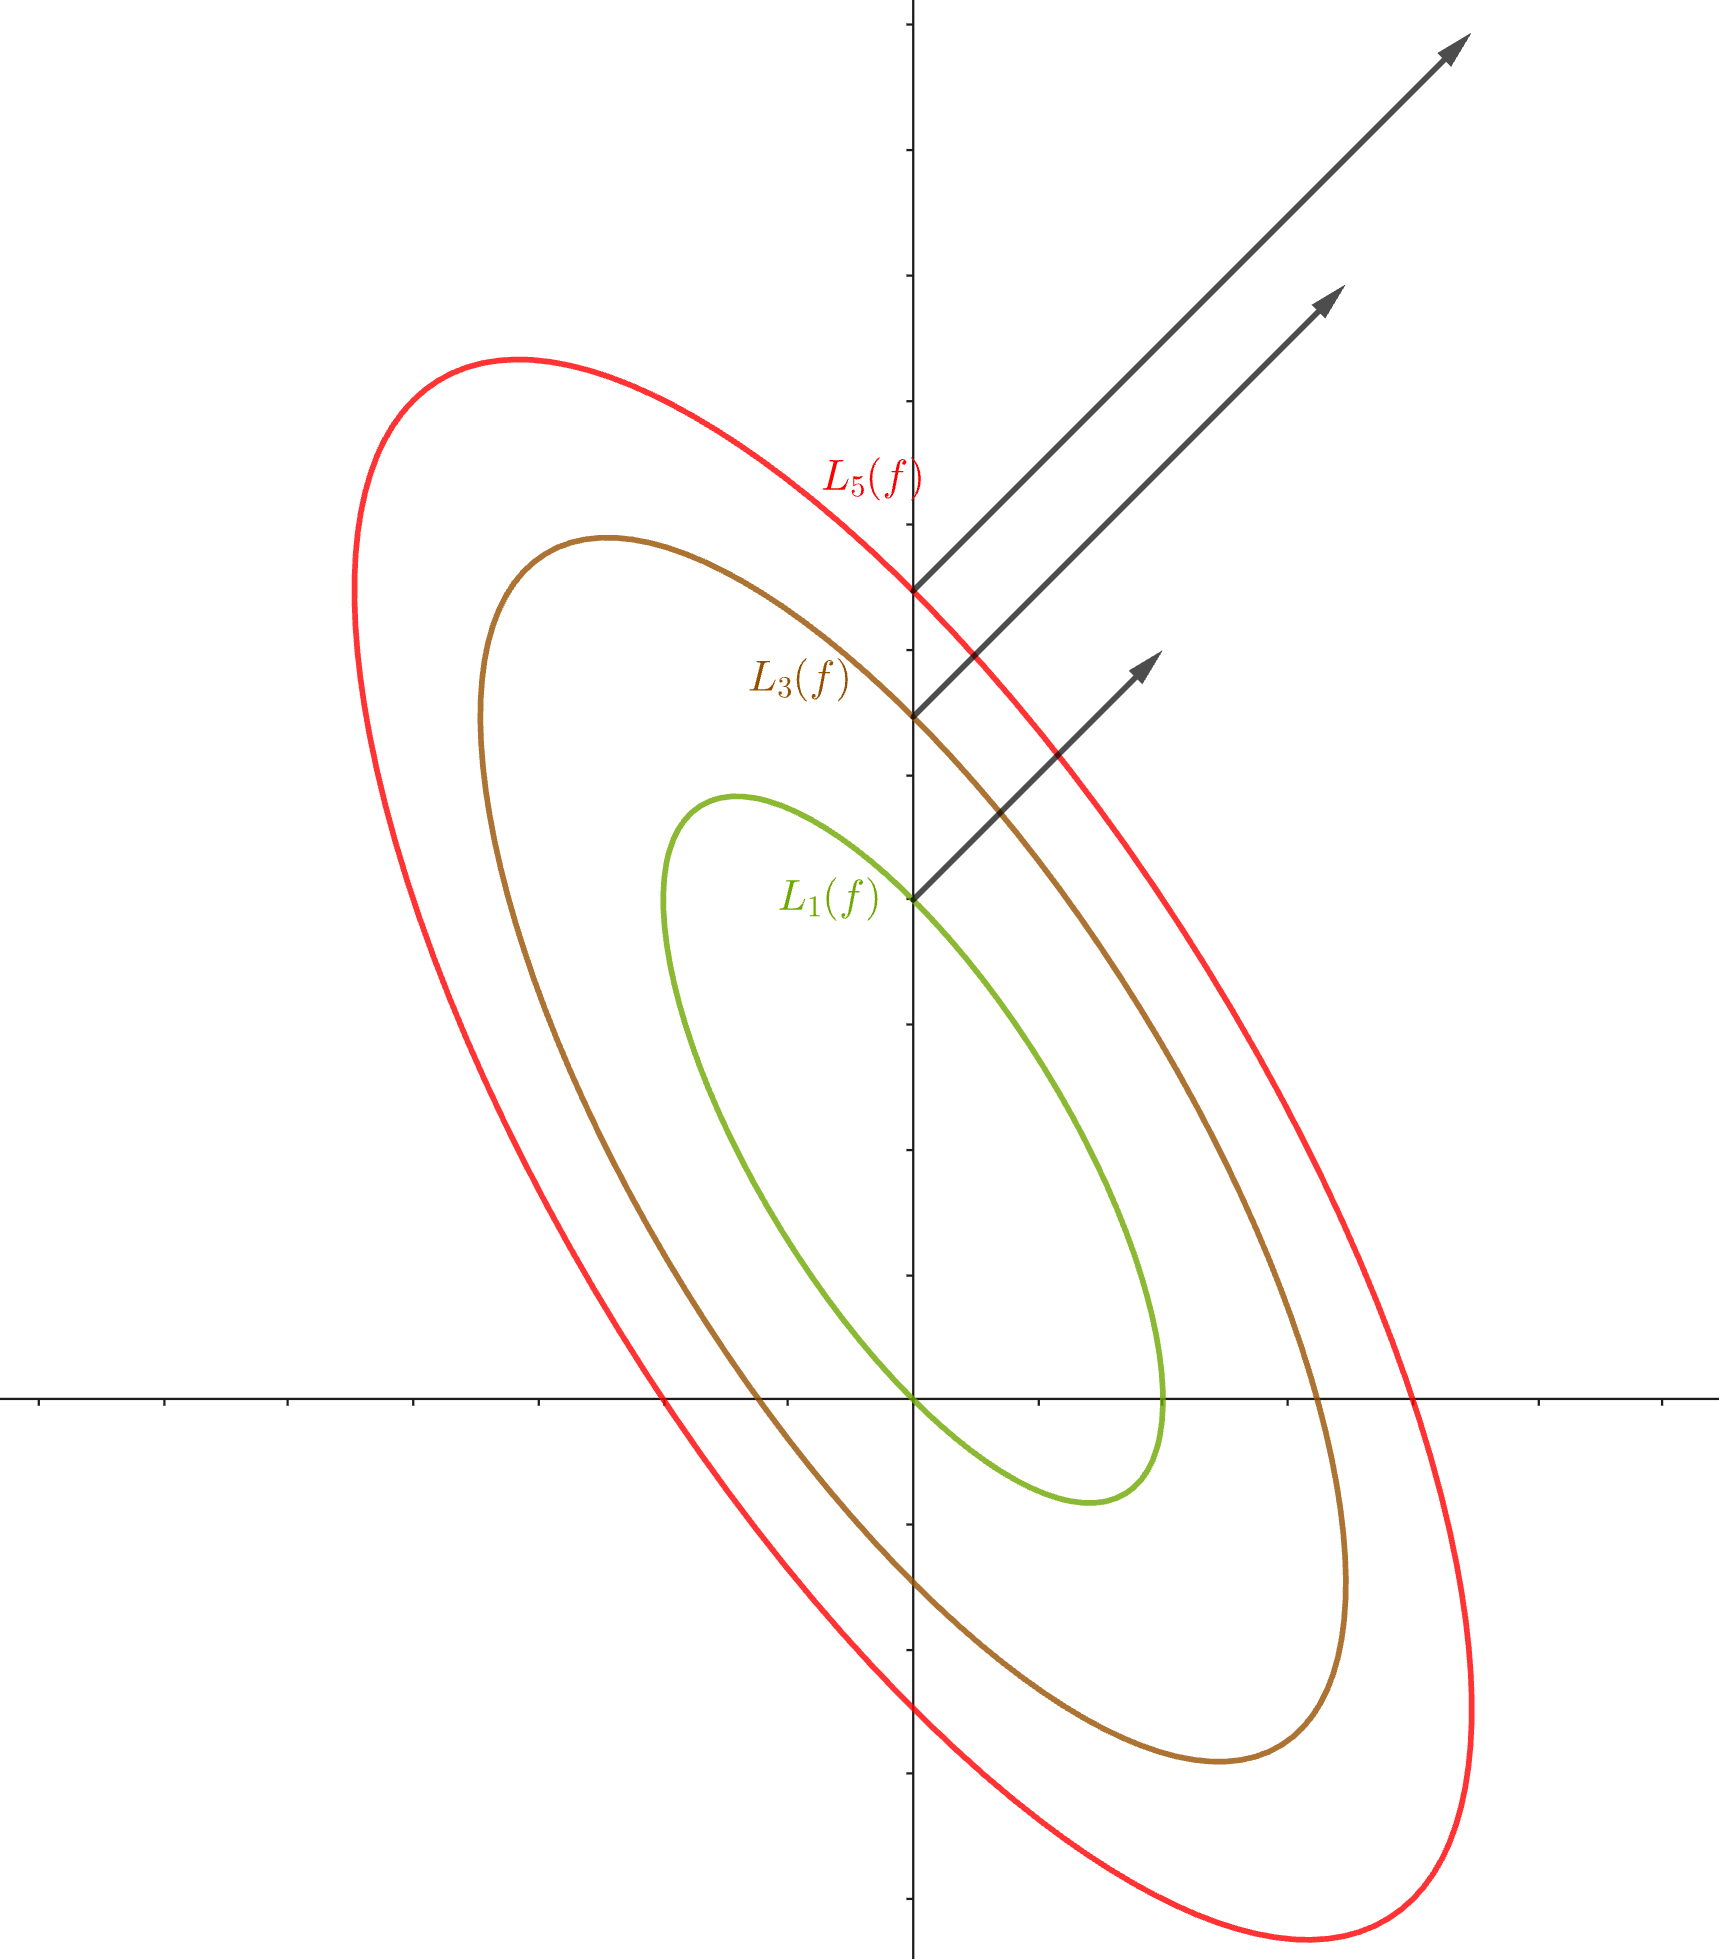
\includegraphics[width=0.5\textwidth]{level.png}
  \caption{Level sets $L_{a}(f)$ and the gradient vector at point $\left(0,1+\sqrt a\right)$ for $a=1,3,5$}
 \end{figure}

The gradient is $\nabla f(x) = \begin{bmatrix}
\frac{\partial f}{\partial x_{1}}\\
\frac{\partial f}{\partial x_{2}}
\end{bmatrix} = 
\begin{bmatrix}
2x_{1}+x_{2}-1\\x_{1}+x_{2}-1
\end{bmatrix}$.

The Hessian is $\nabla^{2}f(x) = \begin{bmatrix}
\partial_{11}f& \partial_{12}f\\
\partial_{21}f & \partial_{22}f
\end{bmatrix} = 
\begin{bmatrix}
2 & 1\\
1 & 1
\end{bmatrix}$. This is a symmetric matrix for $f\in \cC^{2}$, where $\cC^{2}$ is the class of twice differentiable functions with continuous second derivative.

We say a symmetric matrix $H$ is positive definite if $x^{\top}H x > 0 \fa x\ne 0$ and write $H\succ 0$.\\
We say a symmetric matrix $H$ is positive semi-definite if $x^{\top}H x \ge 0 \fa x$ and write $H\succeq 0$.

Why do we care about positive definiteness? Turns out that if $\nabla^{2}f\succ 0$ everywhere, then the function `looks like a cereal bowl'.

This Hessian also turns up in the objective of the $L^{2}$-regression. The objective is \begin{align*}
\frac12\norm{y-Ax}{}^{2} &= \frac12 \left(y^{\top}-x^{\top}A^{\top}\right)\left( y-Ax\right)\\
&= \frac12\left(\norm{y}{}^{2} - 2x^{\top}A^{\top}y  + x^{\top}A^{\top}Ax\right)\\
&=\frac12 \left(\norm y{}^{2}-2x^{\top}A^{\top}y + x^{\top}\nabla^{2}f(x)x\right)
\end{align*} where we used the fact that $\nabla^{2} f(x) = A^{\top}A$ due to the absence of higher order terms and lower than second order terms are differentiated out to $0$. This also tells us that $\nabla f(x) = A^{\top}Ax-A^{\top}y$. If we are at a minima, then we set $\nabla f(x)=0$. This gives $x=\left(A^{\top}A\right)^{-1}A^{\top}y$ if $A^{\top}A$ is invertible. This has a couple of problems. $A^{\top}A$ is huge in the first place, and secondly, inverting a $d\times d$ matrix takes $\cO(d^{3})$ operations and we would like to have smaller computing time.


We have the following gradient descent algorithm: $x_{k+1} = x_{k} - \alpha_{k} \nabla f(x_{k})$. 

Let $\rho(H)$ denote the maximum (in absolute value) of $H$. We have the following theorem that will be stated rigorously and proved next day.

\begin{thm}[informal]
Suppose $\nabla^{2}f(x)\succ 0$ and $\alpha_{k} \le \frac{2}{\rho\left(\nabla^{2}f(x)\right)}$, the above gradient descent algorithm converges `fast'. Otherwise it blows up. 
\end{thm}











%\newpage
%\nocite{*}
%\printbibliography

















\end{document}

